The careful analysis of the experimental data will allow for the calculation of the number of events observed in a specific region of phase space, which combined with the luminosity determined from beam charge accumulated on the Faraday cup provides a rudimentary estimate of the differential \xsec. However, many corrections need to be applied to this raw calculation to arrive at a more accurate result. The most dominant correction term is known as ``acceptance'' which can be thought of the ratio of the number of events that are experimentally detected relative to the number that truly occurred. In this work we will use ``acceptance'' to refer to a combination of geometrical acceptance (the fraction of 4$\pi$ surface area covered by the detector systems), detector efficiency, and track reconstruction efficiency. This correction term (and others) are best estimated by creating a simulation of the physics experiment with computational means, and using the ratio of the number of detected simulated events to the number of generated simulated events as an approximation to the true acceptance, \eqref{eq:acceptance}. 

\begin{equation}\label{eq:acceptance}
    \epsilon_{acc} = \frac{N_{detected,experiment}}{N_{truth}} \approx  \frac{N_{detected,simulation}}{N_{truth,simulation}}  \equiv \frac{N_{sim}}{N_{gen}} = \hat{\epsilon}_{acc}.
\end{equation}

Here $\hat{\epsilon}_{acc}$ is the estimator for the true acceptance, $\epsilon_{acc}$. For the remainder of this work, we will refer to the number of events detected in the real-world experiment as \Nexp, those produced in the real-world as \Ntruth, those detected in the simulation as \Nsim, and those generated for simulation as \Ngen.  

Several components are necessary to arrive at a computational estimate of $\epsilon_{acc}$ and other correction factors. They are: 

\begin{itemize}
    \item A model of the true underlying physics processes to produce \Ngen \secref{sec:ch3generator}
    \item A method to simulate the experiment to produce \Nsim \secref{sec:sim_pipeline}
    \item Sufficient computational infrastructure to perform the calculations \secref{sec:comp_infrastructure}
\end{itemize}



\iffalse
Approaching through the lens of an inverse problem, we use existing knowledge to create event generators that produce reasonable the underlying physics processes. These computer generated datasets are then swam through microphysics simulations of the CLAS12 experiment on an event by event basis to produce a simulated dataset. By comparing the experimental data to the simulated data, and the simulated data to the model of the underlying distribution, inferences can be made about the true underlying distribution generating the experimental data. 
\todo{Fix this stupidly phrased section}
\fi


\section{Event Generation}\label{sec:ch3generator}
    The event generators used in this work are based off the MAID unitary isobar model \parencite{Tiator2006MAIDTechniques}, \parencite{Dreschsel1992ThresholdNucleons} which concerns the photo and electroproduction of pions off of nucleons. It originated as an ``\textbf{A}mplitudes \textbf{A}nd \textbf{O}bservables '' (AAO) generator that worked in the resonance regime \parencite{Burkert1991AmplitudesGenerator} and was extended to function at higher W based off theoretical models \parencite{Goloskokov2010AnElectroproduction} and validated on experimental data \parencite{Bedlinskiy2014ExclusiveCLAS} as well as used in recent physics results \parencite{Diehl2022MultidimensionalRegion}. 

There are two generators, ``aao\_norad'', which is a nonradiative generator that creates events with an outgoing electron, proton, and two photons from the decay of the neutral pion, and ``aao\_rad'', which incorporates radiative corrections into the event generation and produces events with an outgoing electron, proton, neutral pion, and radiated photon. These two generators were refactored to function under a larger software package \href{https://github.com/JeffersonLab/aao_gen}{aao\_gen} which provides access to both generators in one system. Sample distributions of the nonradiative generator are shown in \ref{fig:aao_norad_gen}.

    \begin{figure}[H]
        \centering
        \subfloat{\includegraphics[width=0.5\textwidth]{Chapters/Ch3-Simulations/event_generation/pics/Lepton-Hadron_Angle_phi_vs_Proton_theta,_Gen.png}}
        \hfill
        \subfloat{\includegraphics[width=0.5\textwidth]{Chapters/Ch3-Simulations/event_generation/pics/x_B_vs_Q2,_Gen.png}}
        \caption[Generated Event Distributions]{Generated event distributions}\label{fig:aao_norad_gen}
    \end{figure}


The radiative generator builds off the nonradiative generator to include Radiative Corrections (RC). The generator calculates s-peak and p-peak radiative corrections according to the Mo/Tsai scheme \parencite{MO1969RadiativeScattering}. The calculation produces a radiated photon with a distribution as shown in \figref{fig:aao_rad_mom_distribution}. While more realistic than the nonradiative generator, it also takes roughly 100 times as long to produce events, and so in practice both generators are utilized. 


    \begin{figure}
        \centering
        \includegraphics[trim={0 1.25cm 0 2.5cm},clip,width=0.79\textwidth]{Chapters/Ch3-Simulations/event_generation/pics/radiated_photon_momentum.png}
        \caption[aao\_rad radiated photon momentum distribution]{aao\_rad radiated photon momentum distribution. The horizontal axis is the radiated photon momentum, in units of Gev/c.}
        \label{fig:aao_rad_mom_distribution}
    \end{figure}
    
%AAO rad genreates four particles, an electron (PID 11), proton(PID 2212), radiated photon (22), and produced pion  (111)
    

%// Pi0 leptoproduction in Goloskokov-Kroll (GK) model. The code is currently being tested and implemented in PARTONS framework with additional features. If you plan to use this work in a publication, please use and reference the most recent version of PARTONS in http://partons.cea.fr 
\iffalse
% NOTES FROM VALERY KUBEROSKSKY
Andrey Kim and Nick Markov have the pi0 generator. It has my parametrization for W>2 GeV and MAID for W<1.7 GeV.

My model will for sure work for 12 GeV. It actually very close even for the COMPASS pi0 data (180 GeV muon beam).

There is reasonable coincidence between my model and MAID in the point W=1.7 GeV, not ideal but good enough for the MC.

I think actually that my parametrization has to work in the region W<2 GeV but I am not sure that MAID is doing good job due to the absence the experimental data at W~1.7 GeV. 

%FROM ONE OF THE READMES:
***************************************************************************
*      AUTHOR:        V. BURKERT AND Z. LI
*      FIRST VERSION: SUMMER, 1991.  RECENT UPDATE: MAY.1993
* AO IS WRITTEN BASED ON THE ORIGINAL PROGRAM A_AND_O FROM V.BURKERT
* THIS PROGRAM SHOULD BE LINKED TO EITHER QKMC OR QKXM FOR THE CALCULATION
* OF QUARK MODEL.  
* QKMC AND QKXM USE DIFFERENT FORM FACTORS:
* QKMC USES THE TREATMENT OF FOSTER ET. AL.
* QKXM USES THE DIPOLE FORM FACTOR 
* QKMC IS THE DEFAULT CHOICE IN THIS PACKAGE.
* AO CAN BE USED TO EXAM: Q2-DEPENDENCE OF HELICITY AMP. AT RES. POSITION (GO1)
*                         OUTPUT:GDH.TOP: A B CA(A_1/2) CB(A_3/2)
*                         GDH SUM RULE (GO2):OUTPUT GDH.TOP
*                         OBERVABLES  (RETURN):OUTPUT TEST.TOP
**************************************************************************
*           AO.FOR
* AO CONTAINS THE FOLLOWING SUBROUTINES/FUNCTIONS:
* SIGMA--CALCULATES OBSERVABLES
* EPRES--CALCULATES BREIT-WIGNER RESONANCE AMPLITUDES
* EXPA --CALCULATES THE HELICITY AMPLITUTES FROM EXPT (V.BURKERT ORIGINAL)
* BORNT--CALCULATES THE BORN TERM CONTRIBUTIONS
* BACK --CALCULATES BORN AND NON-BORN BACK GROUND TERMSS
* QKMA --CALCULATES THE HELICITY AMPLITUTES FROM QUARK MODEL
* RAMPF --CALCULATES THE Q2-DEPENDENCE OF THE HELICITY AMP. AT RES. POSITIONS
* HAMP --CALCULATES THE ENERGY-DEPENDECE OF THE RESONANCE HELICITY AMPLITUDES
* QKMC --CALCULATES THE COUPLING CONSTANTS FROM QUARK MODEL
************************************************************************
**************************************************************************
* UPDTATED: NOV., 1992
*         * WITH NEW OPTIONS TO TURN THE BORN TERM ON AND OFF
*         * BORN TERM ARE MODIFIED WITH A CUT OFF FACTOR AT HIGHER 
*           ENERGIES (WCM>1.3 GEV)
*         * SOME CORRECTIONS HAVE BEEN MADE TO THE EXPA SUBROUTINE
***************************************************************************  

 %OTHER GENERATOR NOTES:
    For Exclurad we have similar model, in end may have to iterate a few times to improve the model
    Exlclurad specifically for resonance region, theoretically should be correct, input probably needs to be updated, can put Valery’s new parameterization to cover higher range. Should not be a real issue to implement it because same thing was done for AAORad. High q2 cannot be covered because parameterization only goes to CLAS6 range
    FX: the cruicail thing is to fold in the radiative corrections with acceptance and efficiens. Best mothod is to use fast monte carlo


    aao\_rad and aao\_norad are event generators for exclusive pi0 and pi+ channels with/without radiative effects.  They are written in Fortran.  The program was initially developed by Volker Burkert long time ago for the resonance region, then has been evolved for many years and recently extended to DIS region even though lots of things need to be done.  Try this to see whether it works.  
\fi

\iffalse

    \subsection{Nonradiative Generator}
            Include generator plots, specitics of layout
    

    \subsection{Radiative Generator}
     % Include generator plots, specitics of layout, plots showing W cut offs, etc
    %SANGBAEK PG 76 RC
\fi
   
\clearpage

\section{Simulation Software}\label{sec:sim_pipeline}
 The event generators produce datafiles where each event can be thought of as being represented by 4-vectors (corresponding to the four particles in each event). This represents the (simulated) ground truth of the event. This information must be transformed in a realistic way into the four-momenta typically observed after event reconstruction, data processing, and exclusivity cuts are applied. The most common way to achieve this result is to (1) swim each particle through a physics simulation of the CLAS12 experiment, resulting in simulated detector hits, and (2) pass the simulated detector hit data to reconstruction and analysis algorithms. 

Step (1) is realized through the use of Geometry and Tracking (Geant4) \parencite{Agostinelli2003Geant4aToolkit}, which is a Markov-Chain Monte Carlo (MCMC) software package that simulates the microphyics at each (variable) step along a particle's path through space. This has been implemented for the CLAS12 experiment as a the ``Geant4 Monte Carlo'' (GEMC) software system \parencite{Ungaro2020TheSimulation}, which allows for the simple insertion of CAD models into the Geant4 system, with the basic architecture shown in \ref{fig:gemc_architecture}. 

\begin{figure}[htb]
    \centering
    \includegraphics[width=0.65\textwidth]{Chapters/Ch3-Simulations/simulation_pipeline/pics/gemc_basics.png}
    \caption[GEMC Architecture]{GEMC architecture. Image from \parencite{Ungaro2020TheSimulation}.}
    \label{fig:gemc_architecture}
\end{figure}

Step (2) is straightforward after having been developed as discussed in \chref{Chapter:Experiment}. The distributions from \figref{fig:aao_norad_gen} after passing through the GEMC simulation, CLAS12 reconstruction software, and event selection are shown in \figref{fig:aao_norad_sim}, where the differences between the distributions is indicative of the acceptance cutoffs of the CLAS12 experiment. 


    \begin{figure}[H]
        \centering
        \subfloat[]{\includegraphics[width=0.5\textwidth]{Chapters/Ch3-Simulations/event_generation/pics/x_B_vs_Q2,_rec.png}}
        \hfill
        \subfloat[]{\includegraphics[width=0.5\textwidth]{Chapters/Ch3-Simulations/event_generation/pics/Lepton-Hadron_Angle_phi_vs_Proton_theta,_rec.png}}
        \caption[Reconstructed Event Distributions]{Reconstructed event distributions.}\label{fig:aao_norad_sim}
    \end{figure}

\iffalse
    
    Event generation - fortran and c++ python wrapped
    geant4 docker gemc sysem
    reconstruction from part 2
    
    CLAASana
    
    this should talk about Geant4, GEMC, microphysics MCMC

\fi


    
        



\section{Computational Resources and Infrastructure}\label{sec:comp_infrastructure}
   
    Generating realistic \dvpip events and simulating physics experiments are computationally intensive tasks. Personal computers can run the necessary software, but a sufficient number of simulated events would require an unacceptably long amount of time on a single device. Consequently, much effort has been devoted to the construction of computational centers and corresponding data pipelines to facilitate large scale computing efforts. 

\subsection{Scope of Computations}

    How many simulated events are needed? The simple answer is ``many''. As the number of simulated events grows, the uncertainty of the acceptance estimator $\hat{\epsilon}_{acc}$ (and other computationally derived correction factors) decreases. While simulated data are significantly less expensive than experimental data, they are not free and therefore some realistic bound must be made. As a quick heuristic, it is reasonable to perform enough simulations so as that the uncertainty of the $\hat{\epsilon}_{acc}$ is negligible compared with the other uncertainties of the measurement, or at least is non-dominant. Considering only the acceptance correction in the cross section, \eqref{eq:DVPiPCrossSection_acc_corr}

    
     \begin{equation}\labelAndRemember{eq:DVPiPCrossSection_acc_corr}
           { \frac{    d^4\sigma_{  ep \rightarrow ep'\pi^0}   } {dQ^2dx_Bdtd\phi_{\pi}} 
                =   \frac{ \textcolor{red}{ N(Q^2,x_B,t,\phi_{\pi})}} {\Lumiint \textcolor{purple}{ \Delta \Omega}}
                \frac{1}{\textcolor{correctionfactors}{\epsilon_{acc}}} = \frac{ \textcolor{red}{ N_{exp} }} {\Lumiint \textcolor{purple}{ \Delta \Omega}}  \frac{\textcolor{correctionfactors}{N_{gen}}}{\textcolor{correctionfactors}{N_{sim}}}},
     \end{equation}     

     we have the statistical uncertainty from the experimental and stimulated number of events as \eqref{eq:uncert_sum}

    \begin{equation}\label{eq:uncert_sum}
               { 
               \frac{\delta_{\sigma}}{\sigma} = \sqrt{
                \left(\frac{\delta_{N_{exp}}}{N_{exp}} \right)^2+
                \left(\frac{\delta_{N_{sim}}}{N_{sim}} \right)^2 }               }.
         \end{equation}

    %Note that this equation only discusses the uncertainties due to Nsim Nexp for illustration

    The uncertainty in \Nexp and \Nsim, $\delta_{N_{exp}}$ and $\delta_{N_{sim}}$ respectively, are given by $\sqrt{N_{exp}}$ and $\sqrt{N_{sim}}$, which assumes applicability of a Poisson distribution to the process, commonly known as ``counting statistics'' further discussed in \parencite{Knoll2000RadiationMeasurement}. We can then consider the effect of setting \Nsim = X\Nexp, where X is some multiplicative factor. The expression for the total uncertainty then can be reduced to \eqref{eq:uncert_sum_reduced}

        \begin{equation}\label{eq:uncert_sum_reduced}
               {\frac{\delta_{\sigma}}{\sigma} = \sqrt{ \left( \frac{ \sqrt{ N_{exp}} } { N_{exp}} \right)^2  +  \left( \frac{ \sqrt{ X N_{exp}} } { X N_{exp}} \right)^2     } =  \left(\frac{\delta_{N_{exp}}}{N_{exp}} \right) \sqrt{ \left(1+\frac{1}{X} \right)}}.
        \end{equation} \myequations{Relationship between \Nsim and statistical uncertainty}

    The relationship between the combined statistical uncertainty and the number of simulated datapoints is displayed graphically in \figref{fig:simulation_stats_increase}. Other uncertainties in this measurement are at the 5\%-10\% level (\secref{sec:uncertainty_analysis}) so a reasonable first-pass goal targets the statistical uncertainty due to simulation to sit at the 5\% level, corresponding to a factor X = 10 times more simulated events than experimental events. 
    
    \begin{figure}[htb]
        \centering
        \includegraphics[width=0.8\textwidth]{Chapters/Ch3-Simulations/overview/pics/uncertainty_increase_rectangle.png}
        \caption[Comparison between Experimental and Statistical Counting Uncertainties]{Ratio of magnitudes of statistical uncertainties associated with \Nsim and \Nexp as a function of X = $\frac{N_{sim}}{N_{exp}}$. See \appref{app:f} for more details.}
        \label{fig:simulation_stats_increase}
    \end{figure}

    Preliminary analysis revealed that the total number of \dvpip events from the experimental datasets considered was approximately 500,000 ($\sim$ 200,000 from the inbending configuration, 300,000 from the outbending configuration). This corresponds to requiring $\sim$ 5 million simulated events (passing all levels of reconstruction and exclusivity cuts). The acceptance correction factor was expected to be on the order of 1/20 - 1/100, suggesting the need for several hundred million generated events to be passed through the simulation pipeline. \tabref{table:Generated_Data} displays the simulation allocation scheme implemented in this analysis, with higher statistics assigned to the nominal experiment running parameters, and additional simulations budgeted for variational studies and correction factor determination, as further discussed in \chref{Chapter:BaseAnalysis}.


    \iffalse
    \begin{table}[h]
        \centering
        \begin{tabular}{l|lccc}
            \textbf{Config.} & \textbf{Gen. Type} & \textbf{Background} & \textbf{Nevents (MM)} & \textbf{Purpose} \\ \hline
                & norad & none & 100 & Ineff. Study \\
                & norad & 50 nA & 100 & Ineff. Study / Rad. Corr \\
            In. & rad & 50 nA & 300 & Acceptance Corr. \\
                & rad & 45 nA & 100 & Systematics \\
                & rad & 55 nA & 100 & Systematics \\ \hline
                & norad & none & 100 & Ineff. Study \\
                & norad &  50 nA & 100 & Ineff. Study / Rad. Corr \\
            Out. & rad & 50 nA & 300 & Acceptance Corr. \\
                 & rad & 40 nA & 100 & Systematics \\
             & rad & 40 nA (+1.01) & 100 & Systematics \\
            \hline
            Total & - & - & 1400 & - \\
        \end{tabular}
    \caption{Data for various experimental configurations and conditions.}
    \label{table:experiments}
    \end{table}
    
    \fi
    

    \begin{table}[htb]
        \centering
        \begin{tabular}{c|ccc}
            \textbf{Configuration} & \textbf{Gen. Type} & \textbf{Background} & \textbf{Nevents (MM)} \\ \hline
                & norad & none & 100 \\
                & norad & 50 nA & 300 \\
            Inbending & rad & 50 nA & 300 \\
                & rad & 45 nA & 100 \\
                & rad & 55 nA & 100 \\ \hline
                & norad & none & 100 \\
                & norad &  50 nA & 300 \\
            Outbending & rad & 50 nA & 300 \\
                 & rad & 40 nA & 100 \\
             & rad & 40 nA (+1.01) & 100 \\
            \hline
            Total & - & - & 1800 \\
        \end{tabular}
    \caption[Distribution of Generated Events by Configuration]{Number of events generated for various experimental configurations and conditions. \tabref{table:simulated_data} shows this distribution after simulation, reconstruction, and exclusivity cuts.}
    \label{table:Generated_Data}
    \end{table}


    Optimization studies showed that the most computationally efficient batching scheme was to process batches of 10K events to GEMC at a time, which was the bottleneck in the simulation pipeline at 4.5 - 5 hours per job. The non-radiative (radiative) event generator requires 10 minutes (100 minutes) to produce 10K events, and further processing upon completion of GEMC requires $\sim$ 10 minutes per 10K events. This totals $\sim$ 5 hours (6 hours) per 10K events, corresponding to nearly 1 million core-hours for the required total number of simulations, which would take 8 years of continuous running on a single, high-end, 16 core computer. Instead, computing clusters at MIT, JLab, and around the globe were utilized to realize these computational efforts in a much more reasonable timeframe. 
    


    \iffalse
    \begin{table}[h]
        \centering
        \begin{tabular}{c|ccc}
            \textbf{Configuration} & \textbf{Gen. Type} & \textbf{Background} & \textbf{Nevents (MM)} \\ \hline
                & norad & none & 5 \\
                & norad & 50 nA & 5 \\
            Inbending & rad & 50 nA & 15 \\
                & rad & 45 nA & 10 \\
                & rad & 55 nA & 10 \\ \hline
                & norad & none & 10 \\
                & norad &  50 nA & 10 \\
            Outbending & rad & 50 nA & 30 \\
                 & rad & 40 nA & 10 \\
             & rad & 40 nA (+1.01) & 10 \\
            \hline
            Total & - & - & 1400 \\
        \end{tabular}
    \caption[Distribution of Simulated Events by Configuration]{Number of simulated events for various experimental configurations and conditions.\tabref{table:Generated_Data} shows the corresponding number of generated events per distribution. \textcolor{red}{\textbf{NOTE: Values in this table are placeholders and need to be updated with final figures}}}
    \label{table:simulated_data}
    \end{table}

    \fi



    
    \todo{find some way to include the distribution of ambient radiation (cememnt, etc) - Knoll 767 -  into thesis appendix - include discussion of background merging - not an issue at these scales}


\subsection{MIT Tier 2 and High Throughput Computing}

    The primary computing center utilized for this analysis effort was the MIT Tier 2 cluster, located at the MIT Bates Research and Engineering Center in Middleton, MA, which has 1,088 cores dedicated to CLAS12 computing \figref{fig:BatesComputing}.  Also used for this work was the Massachusetts Green High Performance Computing Center (\href{https://www.mghpcc.org/}{MGHPCC}) in Holyoke, MA. MIT Earth and Planetary Science provides access to these nodes through their \href{https://engaging-ood.mit.edu/pun/sys/dashboard}{Engaging} system, while the MIT Tier 2 cluster is accessible via the \href{https://submit.mit.edu/}{subMIT} system, which also grants users access to a number of other (non-dedicated) computing clusters.

    


    %1,088 cores dedicated to CLAS computing. I believe this means we have 24 hours per day * 1088 cores = ~ 26K core hours per day dedicated   
    %The Bates Laboratory center consists of 71 water-cooled racks, each of which can supply up to 12 kW of power and cooling, and a high-speed 100 Gb/s network link to campus. It uses about 500 kW of power to operate and have 20 petabytes of storage at present.


    \begin{figure}
        \centering
        \includegraphics[width=0.8\textwidth]{Chapters/Ch3-Simulations/overview/pics/Bates_Tier2.jpg}
        \caption[MIT Tier 2]{MIT Tier 2 computing racks at MIT Bates. Image courtesy of E. Ihloff}
        \label{fig:BatesComputing}
    \end{figure}


    
    %and is, which is a larger computational framework that additionally provides access to other computing centers,



    %SUBMIT:     1 TB of free storage per user,     100s of cores and GPUs available interactively and through Slurm     Access to OSG, CMS T3 and T2, LQCD Cluster, and EAPS


    More broadly, the Open Science Grid (OSG) \parencite{OSG2006OSG} \parencite{Sfiligoi2009TheGlideinWMS} \parencite{Pordes2007TheGrid} was leveraged to gain access to dozens of computing clusters around the world. OSG is an organizational system allowing users to utilize idling resources at more than 100 participating institutions, facilitating more than a billion core-hours of computation per year. 

    A significant endeavor in this work was constructing a software bridge connecting the CLAS12 experiment and these computing resources. The effort was realized as the \href{https://gemc.jlab.org/web_interface/index.php}{CLAS12 Simulation Submission Portal} \parencite{Ungaro2020CLAS12Framework}, which established the database back-end, user-friendly front-end \figref{fig:clas12_sub_portal}, and appropriate connection services to interact efficiently with these clusters. 
      
    \begin{figure}[H]
        \centering
        \newlength{\imageheight}
        \settoheight{\imageheight}{\includegraphics[width=0.5\textwidth]{Chapters/Ch3-Simulations/overview/pics/websub_start_narrow_new.png}}
        \subfloat[CLAS12 Submission Portal Main Page]{\includegraphics[width=0.5\textwidth]{Chapters/Ch3-Simulations/overview/pics/websub_start_narrow_new.png}}
        \hfill
        \subfloat[Simulation Sample Webform]{\raisebox{\dimexpr\imageheight-\height}{\includegraphics[width=0.45\textwidth]{Chapters/Ch3-Simulations/overview/pics/websub_lund.png}}}
        \caption[CLAS12 Simulation Submission Portal]{The CLAS12 Simulation Submission Portal, designed to facilitate efficient high-throughput simulations using a variety of generators and experimental configurations.}\label{fig:clas12_sub_portal}
    \end{figure}

    The system is capable of using any event generator on the CLAS collaboration list of \href{https://github.com/JeffersonLab/clas12-mcgen}{officially approved generators} or by passing any internet-accessible folder location of generated event files conforming to the \href{https://gemc.jlab.org/gemc/html/documentation/generator/lund.html}{LUND} standard. As of July 2023, the aao\_gen generators were not yet recognized as officially supported, so event generation had to occur independently of this system, although work is ongoing to recieve offical status. Inferfacing with computing nodes is facilitated through use of Simple Linux Utility for Resource Management (SLURM) \parencite{Yoo2003SLURM:Management} and High Throughput Computing - HTCondor \parencite{HTCondorTeam2023HTCondor} protocols. The system has been succesful, facilitating 85.2 million core-hours of CLAS12 simulations over 2021-2022 as shown in \figref{fig:monthly_hours}.
       
    
    \begin{figure}
        \centering
        \includegraphics[width=0.99\textwidth]{Chapters/Ch3-Simulations/overview/pics/core_hours_2021-22.png}
        \caption[Monthly Core-Hours Utilized at Various Computing Clusters]{Monthly core-hours used for CLAS12 simulations in 2021-22. The portal facilitated 85.2 million core-hours of simulations over the past 2 years.}
        \label{fig:monthly_hours}
    \end{figure}

    Finally, files can be transferred easily from computing clusters to local/personal machines through the use of \href{https://www.globus.org/}{Globus} \parencite{Allen2012SoftwareScientists} \parencite{Foster2011GlobusServices}, or directly through use of ssh protocols. The complete data pipeline for simulations used in this analysis is shown in \figref{fig:simulation_workflow}.


    \begin{figure}
        \centering
        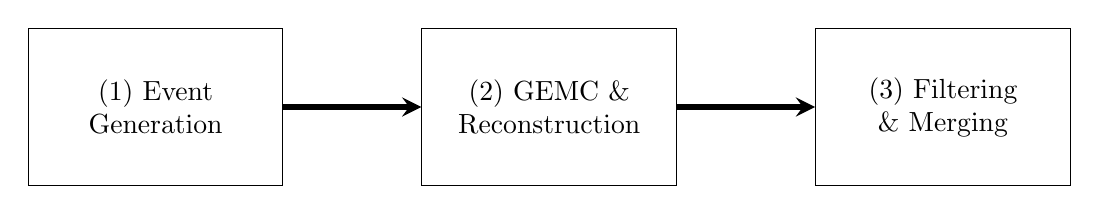
\begin{tikzpicture}[
            box/.style={rectangle, draw, minimum size=2cm, text width=3cm, align=center},
            arrow/.style={->, >=stealth, line width=2pt},
        ]
        
        \node[box] (event) at (0,0) {(1) Event \\ Generation};
        \node[box] (gemc) at (5,0) {(2) GEMC \& \\ Reconstruction};
        \node[box] (filter) at (10,0) {(3) Filtering \& Merging};
        
        \draw[arrow] (event) -- (gemc);
        \draw[arrow] (gemc) -- (filter);
        
        \end{tikzpicture}
        \caption[Event Simulation Pipeline]{Event simulation pipeline. (1) Events are generated using aao\_gen on either MIT Tier 2, MGHPCC, or JLab's SciComp nodes. (2) Events are submitted through the CLAS12 Submission Portal to run on dedicated or idling resources to the GEMC \& CLAS12 event reconstruction suite. (3) Simulated events are returned to JLab's computing nodes, where they are further filtered as discussed in \secref{sec:filtering} and transferred to local computers for analysis.}
        \label{fig:simulation_workflow}
    \end{figure}


    

    \todo{WHERE IS THE JLAB IFARM INFO?}
   
    
    %It includes in addition, a CMS HI simulation and analysis facility, an LHCb Tier-2 computing center, a Hadronic Physics computing center and various smaller contributions. Presently it is located at Bates in Middleton MA.

    %distributed high throughput computing systems - 





    




    
    
    
    %volatile work
    %To cancel all jobs:
    %scancel -u robertej
    
    %To view all jobs:
    %squeue -u robertej

    
    %local of disk utilization statistics: https://clasweb.jlab.org/clas12offline/disk/work/users.html
    




    %is an intercollegiate high-performance computing facility - joint venture between Boston University, Harvard, MIT, Northeastern, and the University of Massachusetts system. - 300 nodes, 10K CPUs, 

 

    
    
    






    

\clearpage

\section{Simulation Enhancements with Normalizing Flows}\label{sec:normflow}
    Placeholder
    %\subsection{Inverse Transforms and Autoregressive Flows}
    Introduce theory of MAFs

\subsection{Exploration of Simulation Speedup with UNMAF}
    Discuss actual work performed



